%
% Copyright 1999, 2007, 2009 Tomás Oliveira e Silva
% Copyright 2018, 2019, 2020, 2021, 2022 Rui Antunes
%
% LaTeX template for theses at University of Aveiro by Rui Antunes.
% https://github.com/ruiantunes/ua-thesis-template
%
% This code is based on the original LaTeX template created by
% professor Tomás Oliveira e Silva.
% http://sweet.ua.pt/tos/TeX.html
%

% Font size possible values are restricted to 10pt, 11pt and 12pt.
\documentclass[11pt,twoside,a4paper,openright]{report}

% Select language (Portuguese, UK English, or US English).
% \input{tex/config/language/portuguese.tex}
% \input{tex/config/language/ukenglish.tex}
\input{tex/config/language/usenglish.tex}

% UA thesis style file.
% Input your scientific area (accounting, arts, economy, education,
% engineering, health, humanities, or sciences).
% Remove the "draft" option for the final document.
\usepackage[engineering,draft]{uathesis}

% Additional packages.
%
% Note that the order that the packages are imported sometimes it
% matters. That is, some packages should be imported before others.
% Otherwise, it may not work correctly.
%
% You may have to add new packages, remove packages, or modify their
% input arguments to obtain the intended functionality.
%

% This package identifies which TeX engine is in use (pdfTeX or LuaTeX).
\usepackage{iftex}

% Input encoding.
% LuaTeX uses UTF-8 encoding by default.
\ifPDFTeX
\usepackage[utf8]{inputenc}
\fi

% Font encoding.
\usepackage[T1]{fontenc}
\usepackage{textcomp}

% Using "Latin Modern" font is better.
% https://tex.stackexchange.com/questions/88368/how-do-i-invoke-cm-super
% http://tug.org/pipermail/macostex-archives/2004-July/006964.html
% https://tex.stackexchange.com/questions/30814/identity-of-latex-default-sans-serif-font/30816
% https://tex.stackexchange.com/questions/66674/when-i-load-multiple-font-packages-which-one-will-win
% https://tex.stackexchange.com/questions/25249/how-do-i-use-a-particular-font-for-a-small-section-of-text-in-my-document
\usepackage{lmodern}

% Select the language.
% The "csquotes" package should be used with the "babel" package.
% https://tex.stackexchange.com/questions/229638/package-biblatex-warning-babel-polyglossia-detected-but-csquotes-missing
\makeatletter
\ifportuguese@use
\usepackage[portuguese]{babel}
\usepackage[style=portuguese,threshold=1]{csquotes}
\else
\ifukenglish@use
\usepackage[UKenglish]{babel}
\usepackage[style=UKenglish,threshold=1]{csquotes}
\else
\ifusenglish@use
\usepackage[USenglish]{babel}
\usepackage[style=USenglish,threshold=1]{csquotes}
\fi
\fi
\fi
\makeatother

\usepackage[%
a4paper,%
% These margins are according to the UA rules.
% http://www.ua.pt/sga/PageText.aspx?id=4630
% left=30mm,%
% right=25mm,%
% bottom=30mm,%
% top=30mm,%
% However, one may want to slightly modify the margins, so there is no
% shift when changing pages in a PDF document viewer.
% https://en.wikibooks.org/wiki/Basic_Book_Design/Margins
left=30mm,%
right=30mm,%
bottom=30mm,%
top=30mm,%
% To show visible frames for the text area and page.
% showframe,%
]{geometry}

% Mathematical utilities.
\usepackage{amsmath}
\usepackage{amssymb}

\ifPDFTeX

% Font type selection in pdfTeX.

% Linux libertine font type.
% https://ctan.org/pkg/libertine
% \usepackage{libertine}
% \renewcommand{\ttdefault}{lmtt}
% \usepackage[libertine]{newtxmath}

\else
\ifLuaTeX

% Font type selection in LuaTeX.
% https://ctan.org/pkg/fontspec
\usepackage{fontspec}

% By default it is used the CMU font:
%   main: CMU Serif
%   sans: CMU Sans Serif
%   mono: CMU Typewriter Text
%   math: Latin Modern Math
%
% Libertinus font is also a nice choice.
% https://github.com/alerque/libertinus
% https://en.wikipedia.org/wiki/Linux_Libertine
% If you want to use Libertinus select:
%   main: Libertinus Serif
%   sans: Libertinus Sans
%   mono: Inconsolata (one monospaced font at your choice)
%   math: Libertinus Math
%
% You may need to install the fonts if they are missing. You can use
% other fonts that are not mentioned here.
% https://www.overleaf.com/learn/latex/Questions/Which_OTF_or_TTF_fonts_are_supported_via_fontspec%3F
%
% \setmainfont{BaskervilleF}
% \setmainfont{CMU Concrete}
\setmainfont{CMU Serif}
% \setmainfont{FreeSerif}
% \setmainfont{Georgia}\renewcommand{\textsc}{\textrm}
% \setmainfont{Libertinus Serif}
% \setmainfont{Linux Libertine O}
% \setmainfont{Noto Serif}
% \setmainfont{Quattrocento}\renewcommand{\textsc}{\textrm}
% \setmainfont{TeX Gyre Bonum}
% \setmainfont{TeX Gyre Pagella}
% \setmainfont{TeX Gyre Schola}
% \setmainfont{TeX Gyre Termes}
% \setmainfont{Times New Roman}\renewcommand{\textsc}{\textrm}
%
% \setsansfont{Arial}
% \setsansfont{Arimo}
% \setsansfont{CMU Bright}
\setsansfont{CMU Sans Serif}
% \setsansfont{CMU Sans Serif Demi Condensed}\renewcommand{\textsf}{\textnormal}
% \setsansfont{Helvetica}
% \setsansfont{Libertinus Sans}
% \setsansfont{Linux Biolinum O}
% \setsansfont{TeX Gyre Heros}
% \setsansfont{Verdana}
%
% \setmonofont{Courier New}
% \setmonofont{Courier Prime}
\setmonofont{CMU Typewriter Text}
% \setmonofont{Inconsolata}
% \setmonofont{Inconsolata}[Scale=0.9]
% \setmonofont{Inconsolata}[Scale=MatchLowercase]
% \setmonofont{Inconsolata}[Scale=MatchUppercase]
% \setmonofont{JetBrains Mono}
% \setmonofont{Latin Modern Mono}
% \setmonofont{Libertinus Mono}
% \setmonofont{Lucida Console}
% \setmonofont{Menlo}
% \setmonofont{Monaco}
% \setmonofont{Ubuntu Mono}
% \setmonofont{Roboto Mono}
% \setmonofont{Source Code Pro}
% \setmonofont{Space Mono}
%
% To use \mathbf{} without errors.
% https://github.com/wspr/unicode-math/issues/556
\usepackage{unicode-math}
\setmathfont{Latin Modern Math}
% \setmathfont{Libertinus Math}

\else
\RequireLuaTeX
\fi
\fi

% Line spacing. The "setspace" package has to be loaded before the
% "hyperref" package to ensure that the links of footnotes are correct.
% https://tex.stackexchange.com/questions/203439/footnotes-misbehaving-in-report-go-to-front-page-but-behave-correctly-in-other-r
\usepackage{setspace}

\usepackage[font=onehalfspacing]{caption}

% To use more colors.
\usepackage[x11names,table]{xcolor}

% To rotate pages.
\usepackage{pdflscape}

% Managing URLs.
\usepackage[hyphens,spaces]{xurl}

% BibLaTeX bibliography. Select the preferred citation style.
% Alternatively, you can configure your own.
% From the "biblatex" documentation: "When using the hyperref package,
% it is preferable to load it after biblatex."
% \input{tex/config/biblatex/authoryear.tex}
\input{tex/config/biblatex/authoryear-comp.tex}
% \input{tex/config/biblatex/numeric.tex}

% Input ".bib" file name with the references.
\bibliography{refs}

% To break URLs. These values are recommended in the "xurl" package.
\setcounter{biburllcpenalty}{100}
\setcounter{biburlucpenalty}{200}
\setcounter{biburlnumpenalty}{100}

% Add a line break before the URL.
% https://tex.stackexchange.com/questions/27953/linebreak-before-url-with-biblatex-alphabetic
\DeclareFieldFormat{formaturl}{\iffieldundef{url}{}{\newline #1}}
\renewbibmacro*{url+urldate}{%
  \printtext[formaturl]{%
    \printfield{url}}%
  \iffieldundef{urlyear}
    {}
    {\setunit*{\addspace}%
     \printtext[urldate]{\printurldate}}}

% Changing master's thesis text.
% https://tex.stackexchange.com/questions/226989/biblatex-changing-key-mastersthesis-to-mphilthesis
\DefineBibliographyStrings{portuguese}{%
  mathesis = {Dissertação de mestrado},
}
\DefineBibliographyStrings{english}{%
  % mathesis = {MSc thesis},
  mathesis = {Master's thesis},
}

% References (citations, images, tables, among others).
% Links cannot break between pages (it is mandatory to manually
% rearrange the text).
% https://tex.stackexchange.com/questions/1522/pdfendlink-ended-up-in-different-nesting-level-than-pdfstartlink
\usepackage[%
breaklinks,%
% draft,%
hidelinks,%
colorlinks,%
linktoc=all,%
% linktoc=page,%
% For debugging.
% allcolors=blue,%
% For final printed version. Choose the colors you want.
allcolors=black,%
linkcolor=black,%
citecolor=blue,%
urlcolor=blue,%
]{hyperref}

% To make the hyperlink put the cursor at the beginning of the figure
% (that is, not in the figure caption).
\usepackage[all]{hypcap}

% The "cleveref" package has to be loaded after the "hyperref" package.
% The "cleveref" has to be loaded after the "amsmath" package to
% correctly reference equations.
% https://tex.stackexchange.com/questions/148699/equation-reference-undefined-when-using-cref-and-packageamsmath
\usepackage[nameinlink,noabbrev]{cleveref}

% Multiple references to the same footnote.
% https://tex.stackexchange.com/questions/10102/multiple-references-to-the-same-footnote-with-hyperref-support-is-there-a-bett
\crefformat{footnote}{#2\footnotemark[#1]#3}

% To create hyperlinks from the footnotes at the bottom of the page,
% back to the occurrence of the footnote in the main text.
% This package conflicts with the "\footcitetext" command from the
% "biblatex" package.
\usepackage{footnotebackref}

% Table footnote.
% https://tex.stackexchange.com/questions/1583/footnotes-in-tables
% From the "tablefootnote" documentation:
% When the document is compiled with LuaLaTeX, hyperlinks in rotated
% content will be misplaced. Use it with caution.
% \usepackage{tablefootnote}

% Header and footer treatment.
\usepackage{fancyhdr}

% To place floats (figures, tables) at fixed position using the
% "\FloatBarrier" command.
\usepackage{placeins}

% To allow tables spanning multiple pages.
% https://texfaq.org/FAQ-longtab
% To prevent longtable breaking in multirow.
% https://tex.stackexchange.com/questions/64956/prevent-longtable-breaking-in-multirow
% A longtable example.
% http://users.sdsc.edu/~ssmallen/latex/longtable.html
\usepackage{longtable}

% To enhance the quality of tables.
\usepackage{booktabs}

% To specify vertical alignment in rows (tables).
\usepackage{array}

% Horizontally centered and right aligned.
% https://tex.stackexchange.com/questions/154958/vertically-centered-and-right-left-center-horizontal-alignment-in-tabular

% Note: the following shortcuts for column alignments are easy to
% memorize. They form a 3x3 square in the QWERTY keyboard layout.

% --- Top (vertical alignment) ---
% Justified.
% p{...}
% Left-aligned.
\newcolumntype{E}[1]{>{\raggedright\arraybackslash}p{#1}}
% Centered.
\newcolumntype{R}[1]{>{\centering\arraybackslash}p{#1}}
% Right-aligned.
\newcolumntype{T}[1]{>{\raggedleft\arraybackslash}p{#1}}

% --- Middle (vertical alignment) ---
% Justified.
% m{...}
% Left-aligned.
\newcolumntype{D}[1]{>{\raggedright\arraybackslash}m{#1}}
% Centered.
\newcolumntype{F}[1]{>{\centering\arraybackslash}m{#1}}
% Right-aligned.
\newcolumntype{G}[1]{>{\raggedleft\arraybackslash}m{#1}}

% --- Bottom (vertical alignment) ---
% Justified.
% b{...}
% Left-aligned.
\newcolumntype{C}[1]{>{\raggedright\arraybackslash}b{#1}}
% Centered.
\newcolumntype{V}[1]{>{\centering\arraybackslash}b{#1}}
% Right-aligned.
\newcolumntype{B}[1]{>{\raggedleft\arraybackslash}b{#1}}

% Extra column with zero width and no padding. This is used to avoid the
% incorrect alignment in the last column.
% https://tex.stackexchange.com/questions/159257/increase-latex-table-row-height
% https://tex.stackexchange.com/questions/68732/vertical-alignment-in-table-m-column-row-size-problem-in-last-column
\newcolumntype{N}{@{}m{0pt}@{}}

% Empty column separator.
% https://texfaq.org/FAQ-fixwidtab
\newcolumntype{O}{@{}}

% To use 2% of the \textwidth as column separator.
\newcolumntype{I}{@{\hskip0.02\textwidth}}

% Multirow in tables.
\usepackage{multirow}

% New lines in multirow cells.
% https://tex.stackexchange.com/questions/331716/newline-in-multirow-environment
\usepackage{makecell}

% To change the itemize character.
\usepackage{enumitem}

% To compact the "itemize" list.
% https://stackoverflow.com/questions/4968557/latex-very-compact-itemize/4974583#4974583
\setlist{itemsep=5pt,topsep=5pt,parsep=5pt,partopsep=5pt}

% To place "longtable" tables at the top of the page.
\usepackage{afterpage}

% Hyphenation throughout the document.
\usepackage{hyphenat}
% To disable hyphenation use the "none" option.
% \usepackage[none]{hyphenat}

% For rotating text with the "turn" command.
\usepackage{rotating}

% To use the "\sfrac" command.
\usepackage{xfrac}

% Disable displaying page number, header and footer on empty pages.
\usepackage{emptypage}

% Colored boxes.
% \usepackage[most]{tcolorbox}

% To force not to break the line after a hyphen. This conflicts with
% latexdiff. Use it with caution.
% https://tex.stackexchange.com/questions/103608/how-to-force-latex-not-to-break-the-line-after-a-hyphen
% \usepackage[shortcuts]{extdash}

% For creating a list of abbreviations.
\usepackage[%
nogroupskip=false,%
nonumberlist=true,%
nopostdot=true,%
% style=alttree,%
style=listdotted,%
% style=long,%
% style=super,%
shortcuts=abbreviations,%
% The "uathesis" style file is already adding the glossary into the
% table of contents.
toc=false,%
]{glossaries-extra}

% To revert \markright, \markboth and \@starttoc related with the
% \MakeUpperCase command. This is required to not mix up with the
% uppercase of chapter headings.
\glsxtrRevertMarks

% To disable all abbreviation hyperlinks.
% https://tex.stackexchange.com/questions/25805/disable-hyperlinks-in-some-entries-for-glossaries
% \glsdisablehyper

% To add links inside captions.
% https://tex.stackexchange.com/questions/30800/gls-inside-caption-without-protect
\robustify{\gls}

% To specify the widest name of the short form of an abbreviation.
% This applies when the "alttree" style is used.
\glssetwidest{123456789012345}

% To specify dotted distance between abbreviation and description.
% This applies when the "listdotted" style is used.
% https://tex.stackexchange.com/questions/17956/dotted-distance-between-acronym-and-description-in-acronymlist-from-glossaries
\setlength{\glslistdottedwidth}{.28\textwidth}

% To remove bold of the short forms in the glossary.
\renewcommand{\glsnamefont}[1]{\normalfont #1}

% To generate the glossary.
% https://tex.stackexchange.com/questions/243750/acronym-glossary-doesnt-appear
\makenoidxglossaries

% Appendices.
% https://ctan.org/pkg/appendix
% https://texfaq.org/FAQ-appendix
% https://tex.stackexchange.com/questions/49643/making-appendix-for-thesis
% Do not use the "page" option if you do not want to create an
% additional page with only the title "Appendices".
\usepackage[toc,page]{appendix}
% \usepackage[toc]{appendix}


% Before begin document.
\input{tex/config/before-begin.tex}

\begin{document}

% After begin document.
\input{tex/config/after-begin.tex}

% First pages.
% Title, Portuguese and English titles, and thesis year.
\newcommand{\authorname}{Carlos Manuel\newline Basílio Oliveira}
\newcommand{\englishtitle}{Towards a scalable Software Architecture for Water Utilities' Decision Support Systems}
\newcommand{\portuguesetitle}{Arquitectura de Software Escalável para Sistemas de Apoio à Decisão para Entidades Gestoras de Água}
\newcommand{\thesisyear}{2022}
% \newcommand{\authorname}{Rui Marcos\newline Brandão Antunes}
% \newcommand{\englishtitle}{\LaTeX\ template for theses at University of Aveiro}
% \newcommand{\portuguesetitle}{Template \LaTeX\ para teses na Universidade de Aveiro}
% \newcommand{\thesisyear}{2022}

% Removing the lines with \setcounter{page} in the titlepage definition
% to disable page numbering restart.
% https://tex.stackexchange.com/questions/68699/how-to-avoid-page-numbering-being-re-started-by-titlepage
% https://tex.stackexchange.com/questions/27543/what-does-the-titlepage-environment-do-and-what-are-its-benefits
% https://www.tug.org/svn/texlive/trunk/Master/texmf-dist/tex/latex/base/report.cls?view=co
\makeatletter
\if@compatibility
  \renewenvironment{titlepage}
    {%
      \if@twocolumn
        \@restonecoltrue\onecolumn
      \else
        \@restonecolfalse\newpage
      \fi
      \thispagestyle{empty}%
      % \setcounter{page}\z@
    }%
    {\if@restonecol\twocolumn \else \newpage \fi
    }
\else
  \renewenvironment{titlepage}
    {%
      \if@twocolumn
        \@restonecoltrue\onecolumn
      \else
        \@restonecolfalse\newpage
      \fi
      \thispagestyle{empty}%
      % \setcounter{page}\@ne
    }%
    {\if@restonecol\twocolumn \else \newpage \fi
     \if@twoside\else
        % \setcounter{page}\@ne
     \fi
    }
\fi
\makeatother

% First pages are numbered A, B, C, ...
% Also, this avoids wrong back references with the biblatex package.
\pagenumbering{Alph}

\begingroup
% Use Helvetica font in the first pages (according to the UA rules).
% https://tex.stackexchange.com/questions/427245/how-to-use-helvetica-font-in-online-editor
% https://www.overleaf.com/learn/latex/Font_typefaces
% In fact the TeX Gyre Heros is used because it can be used as a
% substitute for Adobe Helvetica.

\ifPDFTeX
\renewcommand{\sfdefault}{qhv}
% \renewcommand{\sfdefault}{phv}
\fi

\ifLuaTeX
% \renewfontfamily\sffamily{Arial}
% \renewfontfamily\sffamily{Arimo}
% \renewfontfamily\sffamily{Helvetica}
\renewfontfamily\sffamily{TeX Gyre Heros}
\fi

% Cover page.
\TitlePage
  \HEADER{\BAR}{\thesisyear}
  \vspace*{14mm}
  \TITLE{\authorname}{\portuguesetitle}
  \vspace*{7mm}
  \TITLE{}{\englishtitle}
\EndTitlePage

% Empty page.
\titlepage\ \endtitlepage

% Initial thesis pages.
\TitlePage
  \HEADER{}{\thesisyear}
  \vspace*{14mm}
  \TITLE{\authorname}{\portuguesetitle}
  \vspace*{7mm}
  \TITLE{}{\englishtitle}
  \vspace*{15mm}
  \TEXT{}{Dissertação apresentada à Universidade de Aveiro para cumprimento dos requisitos necessários à obtenção do grau de Mestre em Engenharia Informática, realizada sob a orientação científica do Doutor \mbox{André Zúquete}, auxiliar do Departamento de Eletrónica, Telecomunicações e Informática da Universidade de Aveiro, e do Doutor António Gil
  D’Orey Andrade Campos (co-orientador), Professor auxiliar do Departamento de Engenharia
  Mecânica da Universidade de Aveiro.}
  \vspace*{\fill}
  %\TEXT{}{Apoio financeiro da FCT e do FSE no âmbito do III Quadro Comunitário de Apoio. (se aplicável)}
\EndTitlePage

% Empty page.
\titlepage\ \endtitlepage

\TitlePage
  \vspace*{55mm}
  \TEXT{\textbf{o júri~/~the jury\newline}}
       {}
  \TEXT{presidente~/~president}
       {\textbf{ABC}\newline {\small
        Professor Catedrático da Universidade de Aveiro (por delegação da Reitora da
        Universidade de Aveiro)}}
  \vspace*{5mm}
  \TEXT{vogais~/~examiners committee}
       {\textbf{DEF}\newline {\small
        Professor Catedrático da Universidade de Aveiro (orientador)}}
  \vspace*{5mm}
  \TEXT{}
       {\textbf{GHI}\newline {\small
        Professor associado da Universidade J (co-orientador)}}
  \vspace*{5mm}
  \TEXT{}
       {\textbf{KLM}\newline {\small
        Professor Catedrático da Universidade N}}
\EndTitlePage

% Empty page.
\titlepage\ \endtitlepage

\TitlePage
  \vspace*{55mm}
  \TEXT{\textbf{agradecimentos}}
       {Agradeço o apoio da minha família, amigos e colegas da SCUBIC, e ao prof. Zúquete pela paciência e disponibilidade estes últimos anos}
  \vspace*{5mm}
  \TEXT{\textbf{acknowledgments}}
       {I wish to thank my family, friends and coworkers at SCUBIC for the support, as well as prof. Zúquete for the availability and patience through these past years}
\EndTitlePage

% Empty page.
\titlepage\ \endtitlepage

\TitlePage
  \vspace*{55mm}
  \TEXT{\textbf{Palavras-chave}}{Água, Arquitectura de Software, Sistemas de Apoio à Decisão, Entidades Gestoras de Água}
  \vspace*{5mm}
  \TEXT{\textbf{Resumo}}{O fornecimento de água às populações é um serviço de qualquer grande sociedade, desde o início da Civilização. Hoje em dia, enormes quantidades de água são fornecidas constantemente a residências e indústrias variadas utilizando motores eléctricos acopolados a bombas de água que consomem vastas quantidades de energia eléctrica. Com o recurso a tarifas de electricidade variáveis e dinâmicas, dados em tempo real de sensores nas empresas de fornecimento de água e a modelos da rede de distribuição de água, o software da SCUBIC consegue monitorizar e prever consumos de água e assim optimizar a operação destas bombas por forma a baixar os custos operacionais das empresas gestoras de água.\newline O software fornecido pela SCUBIC é um conjunto de serviços construídos numa fase embrionária da empresa que, por se manterem inalterados ao longo dos anos, não se adequam ao plano de negócios e aumento de requisitos por parte dos \textit{stakeholders}. Daqui surge então a necessidade de construir uma nova arquitectura de software capaz de responder aos novos desafios numa indústria cada vez mais instrumentalizada e evoluída como a da Gestão de Água.\newline Recorrendo a métodos de engenharia de software, migração de arquitecturas de software e planeamento cuidadoso, sugere-se neste trabalho uma nova arquitectura de software baseada em micro-serviços e \textit{serverless}.Esta arquitectura foi então avaliada de acordo com os índices ((indicar quais)) e comparada com a solução antiga. Após rever os resultados gerados pelos indicadores de performance, conclui-se que a migração foi um sucesso.}
\EndTitlePage

% Empty page.
\titlepage\ \endtitlepage

\TitlePage
  \vspace*{55mm}
  \TEXT{\textbf{Keywords}}{Key, word.}
  \vspace*{5mm}
  \TEXT{\textbf{Abstract}}{Water Supply is a staple of all civilizations throughout History. Nowadays, huge amounts of water are constantly supplied to homes and businesses, requiring the use of electric pumps which consume vast amounts of electric energy. \newline By using variable and dynamic electric tariffs, multiple real-time sensor date from Water Utilities and Water Network Modelling, the SCUBIC software is able to monitor the water networks, predict water consumption and optimize pump operation allowing the Water Utilities to lower operational costs.\newline Built during an earlier phase of the company, the SCUBIC software is a monolithic amalgamation of  services, full of compromises that cannot fulfill the latest requirements from the \textit{stakeholders} and business plan. \newline Therefore, a need to build a more modular and scalable software architecture for this software becomes apparent. Using careful planning, software engineering knowledge and literature regarding software architecture migration, a new software architecture was implemented. Results from comparisons between the older and newer architectures prove that the migration was a success and complies with the requirements set at the beginning of the project.}
\EndTitlePage

% Empty page.
\titlepage\ \endtitlepage

% End of Helvetica font.
\endgroup

% Specifying header content. In this case it only shows chapter
% information: left position at even pages, right position at odd pages.
\setlength\headheight{16pt}
\pagestyle{fancy}
\fancyhf{}
\fancyhead[LO,RE]{\fontsize{12}{14.4}}
\fancyhead[LE,RO]{\fontsize{12}{14.4}\textsc{\nouppercase{\leftmark}}}

% To change the font size of the page numbering in all pages.
\fancyfoot[C]{\small\thepage}

% From the "fancyhdr" package documentation.
% "Some LATEX commands, like \chapter, use the \thispagestyle command to
% automatically switch to the plain page style, thus ignoring the page
% style currently in effect."

% The "fancyhdr" packages does not apply same header/footer on chapter
% and non-chapter pages.
% https://tex.stackexchange.com/questions/117328/fancyhdr-does-not-apply-same-header-footer-on-chapter-and-non-chapter-pages

\fancypagestyle{plain}{%
  % Clear all header and footer fields.
  \fancyhf{}
  % Except the center.
  \fancyfoot[C]{\small\thepage}
  \renewcommand{\headrulewidth}{0pt}
  \renewcommand{\footrulewidth}{0pt}
}

% To specify 1x or 1.5x vertical spacing between lines.
% \singlespacing
\onehalfspacing

% Tables of contents, of figures, of tables.

% To count the following pages with roman numbering.
\pagenumbering{roman}

\tableofcontents
\cleardoublepage

\listoffigures
\cleardoublepage

\listoftables
\cleardoublepage

\begingroup
% To locally reduce vertical space between entries.
\setlist{itemsep=0pt,topsep=0pt,parsep=0pt,partopsep=0pt}
\printnoidxglossary
\endgroup
\cleardoublepage

% To specify 1x or 1.5x vertical spacing between lines.
% \singlespacing
\onehalfspacing

% The chapters.

% To count the following pages with Arabic numerals.
\pagenumbering{arabic}


% Chapters.
\chapter{Introduction}\label{intro}




\section{Water Supply Systems}\label{intro:s:water-supply-systems}

The water supply systems that are prevalent in modern society play a very important role in daily life, distributing water throughout the country from water reservoirs or water treatment plants to the citizen's houses and industries. These \glspl{wss} can be quite complex and difficult to manage without proper processes that ensure the efficient operation of such networks including its environmental and economical sustainability. For this reason nowadays, the use of specialized software to aid operators or even automatically control the operation of these \glspl{wss} is of uttermost importance. It must be highlighted that water has been a staple of all major human civilizations throughout History, from ancient roman aqueducts to the current era.

Moving large quantities of water through large \glspl{wss} requires the use of large quantities of mechanical work, which in turn requires high levels of electric energy. With the ever-growing political, economic and environmental pressure to improve and optimize the use of energy, and with the current geopolitical issues, the access to energy is getting more expensive and regulated. This means that the need for the optimization of pumping operations to reduce costs and, potentially reduce the energy use as well, is growing within \glspl{wu}.

\section{Existing Decision Support System}\label{intro:s:existing-decision-support-system}

In order for the \gls{wu}'s water pumps' optimal operation, a \gls{dss} is used by the \gls{wu}'s pump operators and/or by automatic \gls{scada} systems. Generally, this \gls{dss} is a web platform designed to suggest \textit{which} pumps to operate, \textit{when} to operate, for \textit{how} long to operate and in some cases what \textit{speed} their \glspl{vsd} should operate, as shown in \Cref{fig:sanepar-example-01}. This figure is an example from one of SCUBIC's\footnote{https://scubic.tech\label{foot:scubic}} Clients.

\begin{figure}[!htbp]
    \centering
    \fbox{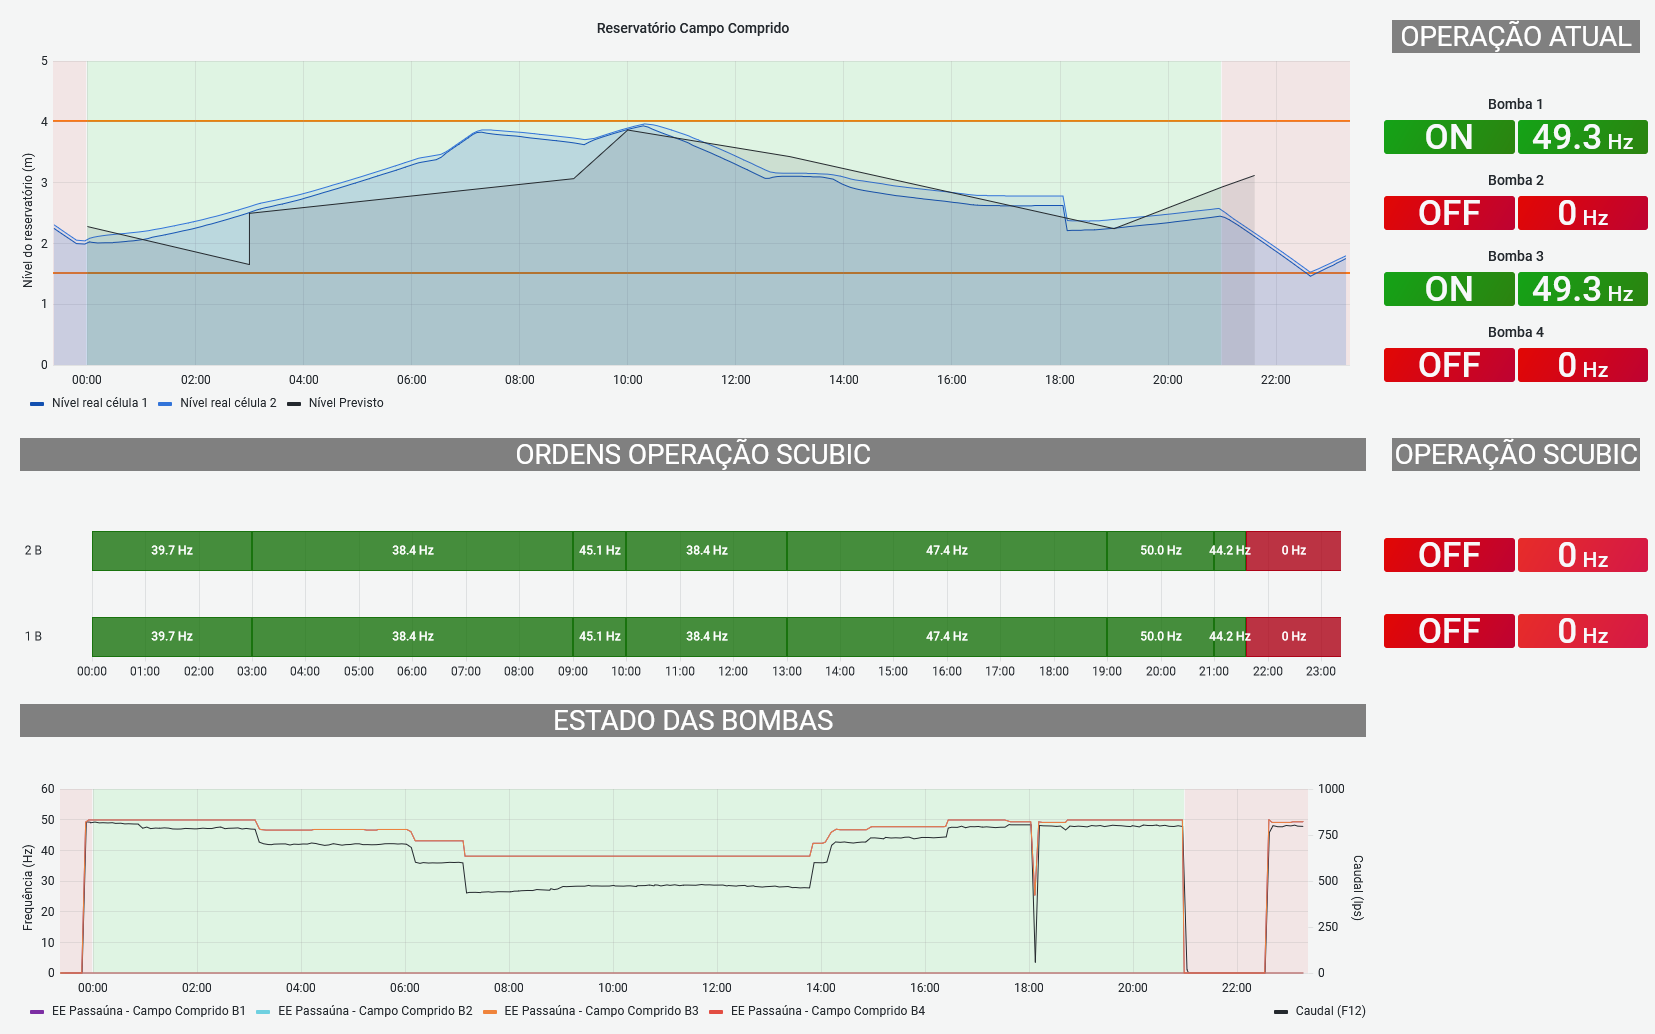
\includegraphics[width=0.95\textwidth]{img/screenshots/sanepar-example-01.png}}
    \caption[DSS example.]{Example of a \gls{dss} interface from one of SCUBIC's Clients}
    \label{fig:sanepar-example-01}
\end{figure}
    

The existing software’s architecture can be summarized as a “Monolithic Modular” software architecture \parencite{newman2019monolith}. This architecture is composed of a set of \glspl{vps}, one for each Client, where a set of Docker containers enclose all the services needed for running the software for that Client. These services are also configured and developed separately, each in a different code repository. This fact results in an unsurmountable amount of \textit{code drift} between the same services of the different clients. \textit{Code drift} happens when, despite being based on the same code, the codebases for each Client follow different paths during software development. When there is a need to implement a new feature or fix a bug common to both codebases, these differences increase the amount of work. Apparently, this structure is not even remotely manageable for any software development team. On \Cref{methodology:s:the-old-architecture}, a complete analysis of this architecture is provided and explained in detail.


\section{Objectives}\label{intro:s:objectives}

The main goal of this work is to make the migration from the old software architecture of the \gls{dss} to a more efficient, improved software, considering the requirements from the \textit{stakeholders} while also improving the cost-performance ratio of the software without compromising the software's functionality.
This new architecture improves the performance, reliability, resilience, security, scalability and observability in comparison to the old \gls{dss} Architecture. The new software architecture brings improvements not just for the software itself but also for the development team, allowing them to improve and maintain the software easier and faster than ever before. By reducing the amount of work and time the software development team spends on each maintenance action or new functionality, it reduces cost to the software company as well. Infrastructure costs are also an important aspect of this new architecture, where the adoption of more modular and independent services means a more optimal use of compute resources, resulting in lowering such costs. This new architecture also improves the Observability of the entire system, allowing for quicker failure detection and to anticipate possible future problems with the system.

As such, the objectives can be summarized as three goals: Enable scalability of the software (through multi-tenancy), improve DevOps' \glspl{kpi} and improve the Observability of the systems.


\section{Structure of the Document}\label{intro:s:structure-of-the-document}

This document is composed by a total of 5 chapters.

In \Cref{intro}, the chapter presents the overall theme of this body of work. Firstly, some context is given about the overall theme of this body of work and the motivation behind it. Then, the objectives for dissertation are presented to the reader. Finally, at the end of the chapter, some information regarding the content of each chapter is presented.

In \Cref{state-of-the-art}, a bibliographical analysis is presented, divided into three parts. Firstly, it's presented a summary of the state-of-the-art on software architecture, cloud-based software solutions, scalability and containerization of services. Secondly, some concepts regarding DevOps' origins and it's influence in today's software development paradigm are presented as well as what \glspl{kpi} are regarded as important for DevOps. Thirdly, Observability is studied and presented, exploring how it can improve software development in general and how it enables the developers and maintainers to gain insight into the system internal state. Additionally, some text regarding the general technologies used throughout the work is also analyzed whenever relevant to the topic in question.

\Cref{methodology} is divided into two sections. Firstly, a more detailed explanation of the old architecture and its inherent flaws is presented. These flaws, which end up showcasing the need for a new and improved software architecture, are related to the objectives established in \cref{intro:s:objectives}. In this section, it's explained how the old software architecture is flawed and has problems with scalability, poor DevOps performance and low-to-non-existent Observability. Then, in a second section, the author proposes a new software architecture that attempts to solve the problems aforementioned. In this later section, it's shown how the new architecture works, it's key components and given multiple diagrams that help explain said architecture. For each one of the flaws presented in the section before, it's presented how each aspect of the new architecture solves those flaws and the reasoning behind the choices that lead to this new architecture. The procedures taken, the challenges and decisions made throughout the implementation are shown and contextualized in this section.

\Cref{results-and-discussion} analyzes how the new architecture manages to achieve the objectives set in the introductory chapter of this document. Firstly, a cost-rundown report and simulated costs are shown that prove the cost-effectiveness improvement. Secondly, it shows how, by using the new architecture, the DevOps' \glspl{kpi}s have improved. Lastly, an overview of the result of implementing changes to the architecture to increase system observability and how it relates to better error detection and increases the system's behavior awareness.

\Cref{conclusion} discusses the previous results and presents some conclusions from what has been demonstrated on previous chapters.

Furthermore, attached to this document, is an appendix that contains some extra results generated from the monitoring interface used internally to evaluate the new architecture.

% \subsection{Options}
% \label{c1:ss:options}

% The following options are supported:

% \begin{itemize}

% \item
% \texttt{oldLogo}: to use the old logo of University of Aveiro.

% \item
% \texttt{newLogo}: to use the new logo of University of Aveiro (default behavior).

% \item
% \texttt{MAP}: for MAP joint doctoral programmes. The logos from the three universities (Aveiro, Minho, Porto) are used.

% \item
% \texttt{draft}: it prints ``DOCUMENTO PROVISÓRIO'' in the first two front pages.

% \item
% \texttt{draftPT}: same as \texttt{draft}.

% \item
% \texttt{draftEN}: same as \texttt{draft}, but instead it prints ``DRAFT DOCUMENT''.

% \item
% As of May 29, 2021, the department name shall not appear in the cover and the first page (top header).
% A new option, \texttt{NODEPT} (no department), was created to suppress the department name (now this is the default behavior).\\
% However, formerly the department name would appear in the cover and first page, therefore the old options were kept for the sake of preservation.
% Any department name can be shown by using one of the following options: \texttt{DAO}, \texttt{DBIO}, \texttt{DCM}, \texttt{DCSPT}, \texttt{DECA}, \texttt{DECIVIL}, \texttt{DEGEIT}, \texttt{DEM}, \texttt{DEMAC}, \texttt{DEP}, \texttt{DETI}, \texttt{DFIS}, \texttt{DGEO}, \texttt{DLC}, \texttt{DMAT}, \texttt{DQ}.

% \item
% The color of the top bar, in the cover page, is defined by specifying one of the following scientific areas: \texttt{accounting}, \texttt{arts}, \texttt{economy}, \texttt{education}, \texttt{engineering}, \texttt{health}, \texttt{humanities}, \texttt{sciences}.

% \end{itemize}

\chapter{State-of-the-Art}\label{state-of-the-art}


\section{Software-as-a-Service}\label{state-of-the-art:s:software-as-a-service}
(( 1 ou 2 parágrafos sobre SaaS e história))

\section{Software Engineering}\label{state-of-the-art:s:software-engineering}

\subsection{Defining Requirements}\label{state-of-the-art:ss:defining-requirements}

Here, we will show what's the state-of-the-art regarding requirements definition. This is an important step in Software Engineering, or any Engineering. 

Deciding on what and how to develop software is a difficult part of the software development cycle \parencite{pacheco_garcía_reyes_2018}.

\subsubsection{Identifying Key Stakeholders}\label{state-of-the-art:sss:identifying-key-stakeholders}

Before requirements elicitation, one of the most important steps is asking from whom should such requirements be elicited from. This step is crucial to prevent functional (and financial) success of the project about to be started \parencite{lewellen_2020}. Requirements elicitation should be performed during the early stages of the software planning phase in order to prevent



\section{Software Architecture}\label{state-of-the-art:s:software-architecture}

(( Que tipos de arquitecturas de software existem ))

\section{Code Deployment}\label{state-of-the-art:s:code-deployment}

\subsection{DevOps}\label{state-of-the-art:ss:devops}

The \textit{portmanteau} of Development and Operations - DevOps - is as "(...) a set of practices intended to reduce the time between committing a change to a system and the change being placed into normal production, while ensuring high quality", according to \parencite{bass_weber_zhu_2015}. There are, therefore, three things to retain from this definition. The two time periods where Development and Deployment occur, the quality of the changes to be committed to a system and the quality of the processes of putting those changes into production.

\subsubsection{Development Time}
This time 






Sallin et.al. \parencite{sallin_kropp_anslow_quilty_meier_2021}

\section{Cloud-Based}\label{state-of-the-art:s:cloud-based}

\subsection{Evaluating Architectures}\label{state-of-the-art:ss:evaluating-architectures}
\chapter{Methodology}
\label{methodology}

\section{Requirements}
\label{methodology:s:requirements}

\subsection{Current Architecture}
\label{methodology:ss:current-architecture}

The current software architecture is still in use as of the date of publication of this body of work. This older architecture consists of an amalgamation of Docker containers, each running a different service. Each Client has its own \gls{vps} wherein these Docker containers are deployed. 

\subsubsection{\gls{vpc}}
\label{methodology:sss:vpc}

These \gls{vps} are general-purpose \gls{aws} \gls{ec2} \textit{Instances}. As can be seen on the diagram presented on \Cref{fig:old-arch-overview.drawio.pdf}, these instances are deployed to the same \gls{vpc}, sharing a private network between them. The Reverse Proxy serves as, as the name implies, as a reverse proxy to enable the use of a single \gls{eip}, a single \gls{nic} by all Clients's servers, since the availability of public IPs is limited to five \gls{eip}.
\begin{figure}[!htbp]
    \centering
    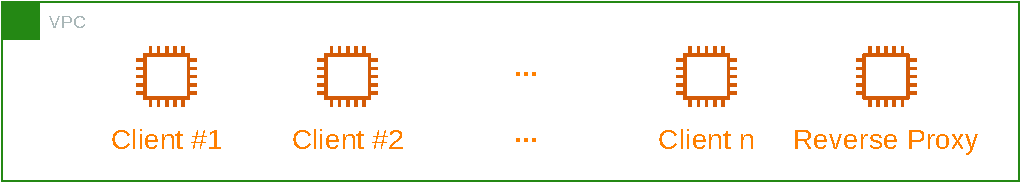
\includegraphics[width=0.90\textwidth]{img/diagrams/pdf/old-arch-overview.drawio.pdf}
    \caption[AWS VPC Overview]{The AWS VPC used, hosting the old architecture's EC2 \gls{vps}.}
    \label{fig:old-arch-overview}
\end{figure}
    

\subsubsection{\gls{vpc}}
\label{methodology:sss:vpc}

Each \gls{ec2} instance runs a Docker container for each one of the following services:

\begin{itemize}

\item \textbf{InfluxDB} (Timeseries Database)
\item \textbf{MongoDB} (General use, no-SQL, Document Database)
\item \textbf{Grafana} (Web platform for data visualization, the front end of the \gls{dss})
\item \textbf{Telegraf} (Data collecting service)
\item \textbf{Nginx} (Reverse proxy with HTTPS capabilities)
\item \textbf{Let's Encrypt} (Automatic SSL Certificate emitter, companion for the Nginx container)
\item \textbf{Web Dev} (Web platform / API for managing Workers' settings)
\item \textbf{Redis} (Message Queue System for queuing Worker's jobs)
\item \textbf{OpenSSH} (\textit{atmoz/sftp}) (SFTP Server for receiving client data)
\item \textbf{Workers} (Container running the Forecast, Simulation and Optimization Python Algorithms as well as the KPI Algorithms.)
\item \textbf{Workers} (\textit{Beat}) (Container that periodically \textit{triggers} jobs in the Workers container)

\end{itemize}

\begin{figure}[!htbp]
    \centering
    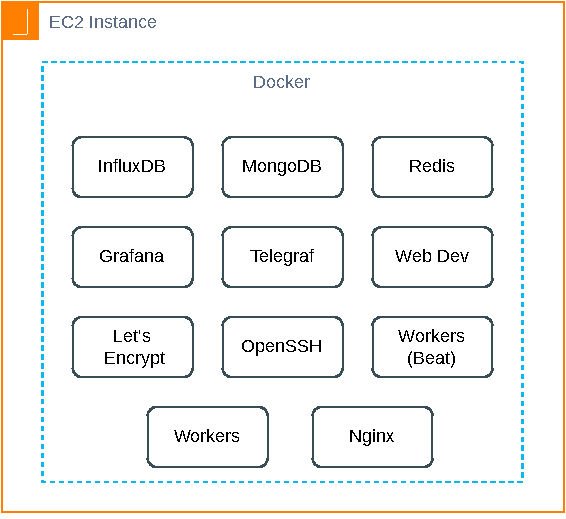
\includegraphics[width=0.75\textwidth]{img/diagrams/pdf/old-arch.drawio.pdf}
    \caption[AWS EC2 VPS Overview]{An AWS EC2 VPS, hosting the old architecture's docker containers}
    \label{fig:old-arch.drawio.pdf}
\end{figure}
    


\subsubsection{Databases}
\label{methodology:sss:databases}

There are two types of databases being used by this architecture: A Timeseries Database, in this case \textbf{InfluxDB}, and an additional general-purpose Document Database: \textbf{MongoDB}. Each type of database has a different role, the first one stores the Client's timeseries data such as sensor information, pump orders, predicted tank levels, etc.
The second one, the Document Database, is responsible for storing configuration settings for each worker service (optimization, simulation and forecasting), for storing electrical tariffs data and to store sensor device's configurations.

\subsubsection{Grafana}
\label{methodology:sss:grafana}

This web platform allows the visualization of the Timeseries data from the \textbf{InfluxDB} database. This is a freely-available platform that runs on a docker container with little to no modifications necessary. The dashboards are built using the built-in tools and allow for complex and very informative data visualization. This is used in both the new and old architecture, since the new visualization platform is still not operational (not within the scope of this body of work).

\subsubsection{Telegraf}
\label{methodology:sss:telegraf}

The \textbf{Telegraf} container is used to gather the files containing the raw sensor data sent from the Client to the \textbf{SFTP} server. Since this container shares the file upload location folder with the \textbf{SFTP}, through a convoluted process of storing the filename of the last file uploaded, periodically checking for the next file and file handling \textit{spaghetti} code that spans multiple files and has an enormous codebase that weighs the docker image's file size considerably. 
\chapter{Results and Discussion}\label{results-and-discussion}

\textcolor{red}{The following structure is not finalized, but should give a good notion of what this chapter will contain}

\section{Architectural Improvements}\label{results-and-discussion:s:architectural-improvements}

\subsection{Overview}\label{results-and-discussion:ss:overview}

\textcolor{orange}{Here, show the overall impact of the new architecture}

\subsection{Cost Rundown}\label{results-and-discussion:ss:cost-rundown}

\textcolor{orange}{Here, show tables and graphs comparing the old and new arch's costs (CAPEX and OPEX and others), together with the scaling part}

\subsection{FKMs}\label{results-and-discussion:ss:fkms}

\textcolor{orange}{Here, show how the new arch improves on the four key metrics for DevOps}

\subsection{Observability}\label{results-and-discussion:ss:observability}

\textcolor{orange}{Here, show some dashboards of the observability system, exemplifying normal day-to-day operation, error detection, etc...}


\chapter{Conclusion}\label{conclusion}

\textcolor{red}{Here, repeat what is said in the introduction and abstract, basically}
\input{tex/contents/c1.tex}
\chapter{Tips and examples}
\label{c2}

This chapter presents some basic tips and a few examples on how to use \LaTeX.


\section{\TeX\ engines}
\label{c2:s:latex-engines}

There are several \TeX\ engines.
In short, these are used to compile the (La)TeX source code to generate the output file (for example, a \as{pdf}).
To know more about these, I encourage you to check these articles:

\begin{itemize}
\item
The TeX family tree: LaTeX, pdfTeX, XeTeX, LuaTeX and ConTeXt.\\
\url{https://www.overleaf.com/learn/latex/Articles/The_TeX_family_tree:_LaTeX,_pdfTeX,_XeTeX,_LuaTeX_and_ConTeXt}

\item
Choosing a LaTeX Compiler.\\
\url{https://www.overleaf.com/learn/latex/Choosing_a_LaTeX_Compiler}

\item
Are there benefits to use XeTeX or LuaTeX if one is to write documents mainly in English?\\
\url{https://tex.stackexchange.com/questions/548467/are-there-benefits-to-use-xetex-or-luatex-if-one-is-to-write-documents-mainly-in}

\item
Why choose LuaLaTeX over XeLaTeX.\\
\url{https://tex.stackexchange.com/questions/126206/why-choose-lualatex-over-xelatex}

\item
Differences between LuaTeX, ConTeXt and XeTeX.\\
\url{https://tex.stackexchange.com/questions/36/differences-between-luatex-context-and-xetex}

\end{itemize}

In this template, support for both pdf\TeX\ and Lua\TeX\ engines has been guaranteed, but I encourage you to use the latter because it is more powerful for typefaces: it supports TrueType and OpenType standards.


\subsection{Compiler automatic detection}

\ifPDFTeX
{\color{red} pdf\TeX\ is being used.}

Consider changing to Lua\TeX, which is the recommended compiler for this template.
\fi

\ifLuaTeX
{\color{Green4} Lua\TeX\ is being used.}

You are using the recommended compiler.
\fi


\section{Basic tips}
\label{c2:s:basic-tips}

\begin{itemize}
\item
The \verb+\\+ command has the same effect as \verb+\newline+.
\item
The \verb+\cleardoublepage+ command forces the next content to start in an odd page.
\item
The tilde character (\verb+~+) inserts a non-breaking space.
Use it before citing a reference to avoid breaking the line: \verb+an example~\cite{label}+.
\item
The current font size is \myfontsize.
\item
Use the \verb+longtable+ environment for tables spanning multiple pages.
\item
The grave accent \`{} and the apostrophe \textquotesingle\ are the correct symbols to make quotations: ``this is an example''.
\end{itemize}


\section{Font styles}
\label{c2:s:font-styles}

\begin{itemize}
\item
\verb+\textnormal{}+ --- \textnormal{document font family}.
\item
\verb+\textrm{}+ --- \textrm{roman font family}.
\item
\verb+\textsf{}+ --- \textsf{sans serif font family}.
\item
\verb+\texttt{}+ --- \texttt{teletypefont family}.
\item
\verb+\textit{}+ --- \textit{italic shape}.
\item
\verb+\textsl{}+ --- \textsl{slanted shape}.
\item
\verb+\textsc{}+ --- \textsc{small capitals}.
\item
\verb+\textbf{}+ --- \textbf{bold}.
\end{itemize}


\section{Colors}
\label{c2:s:colors}

{\color{red} Red colored text} from the \texttt{color} package.
{\color{Blue4} And Blue4 colored text} from the \texttt{xcolor} package.

\section{Footnotes}
\label{c2:s:footnotes}

This is a labeled footnote\cref{foot:example}.
A footnote can be referenced multiple times\footnote{\label{foot:example}This is a footnote example.}.
Again, the same footnote is referenced\cref{foot:example}.


\subsection{A table example}
\label{c2:ss:a-table-example}

A table example is shown in \Cref{tab:a-table-example}.

%\input{tex/contents/tab/a-table-example.tex}


\section{Abbreviations}
\label{c2:s:abbreviations}

\verb+\gls{label}+ and \verb+\glslink{label}{text}+ are two possible commands for making use of abbreviations.
For example, the commands \verb+\gls{afk}+ (first call), \verb+\gls{afk}+ (second call), and \verb+\glslink{afk}{insert specific text}+ produce respectively ``\gls{afk}'', ``\gls{afk}'' and ``\glslink{afk}{insert specific text}''.

A list of some commands follow.

\begin{itemize}
\item
\verb+\gls{afk}+ produces ``\gls{afk}''.
\item
\verb+\glslink{afk}{text}+ produces ``\glslink{afk}{text}''.
\item
\verb+\glsxtrshort{afk}+ and \verb+\as{afk}+ produce ``\glsxtrshort{afk}'' and ``\as{afk}'', respectively.
\item
\verb+\glsxtrlong{afk}+ and \verb+\al{afk}+ produce ``\glsxtrlong{afk}'' and ``\al{afk}'', respectively.
\end{itemize}

Note that the commands \verb+\as{}+ and \verb+\al{}+ are shorter variants.

Other abbreviations include: good work (\as{gw}); have fun (\as{hf}); good work and have fun (\as{gwhf}).
Note that the latter contains nested abbreviations.


\section{Equations}
\label{c2:s:equations}

\Cref{eq:example1} is a numbered equation.

\begin{equation}
\label{eq:example1}
x = 1 + y
\end{equation}

The following equation is not numbered, and thus cannot be referenced.

\begin{equation*}
y = \sum_{i=1}^{N}{x_i}
\end{equation*}

The \verb+\myscore+ pre-defined math function is used by the \Cref{eq:example2}.

\begin{equation}
\label{eq:example2}
\myscore(d) = \frac{1}{d^2}
\end{equation}


\section{Figures}
\label{c2:s:figures}

An example of a figure is shown in \Cref{fig:aveiro}. The \verb+\fbox+ command \fbox{draws a box} around its content.

\input{tex/contents/fig/aveiro.tex}


\section{Rotating pages}
\label{c2:s:rotating-pages}

Horizontal pages can be obtained using the \verb+landscape+ environment  from the \verb+pdflscape+ package:

\begin{verbatim}
\begin{landscape}
Add some text or figures.
\end{landscape}
\end{verbatim}


\section{A long table}
\label{c2:s:a-long-table}

\Cref{tab:a-long-table} presents a long table using the \verb+longtable+ package.
This table can span multiple pages.
The \verb+\afterpage+ command forces the table to start at the top of a page.

\afterpage{\input{tex/contents/tab/a-long-table.tex}}

\input{tex/contents/c3.tex}
\input{tex/contents/c4.tex}

% Bibliography.

% To cite all the references (debugging purposes).
% \nocite{*}

% The bibliography using BibLaTeX.
\printbibliography

% Appendices.
\begin{appendices}
\crefalias{chapter}{appendix}
\chapter{Appendix example}
\label{a1}

\section{Logging Interfaces}

\subsection{Google Cloud's Log Explorer (Former Stackdriver)}\label{a1:ss:google-cloud-log-explorer}
\begin{figure}[!htbp]
    \centering
    \fbox{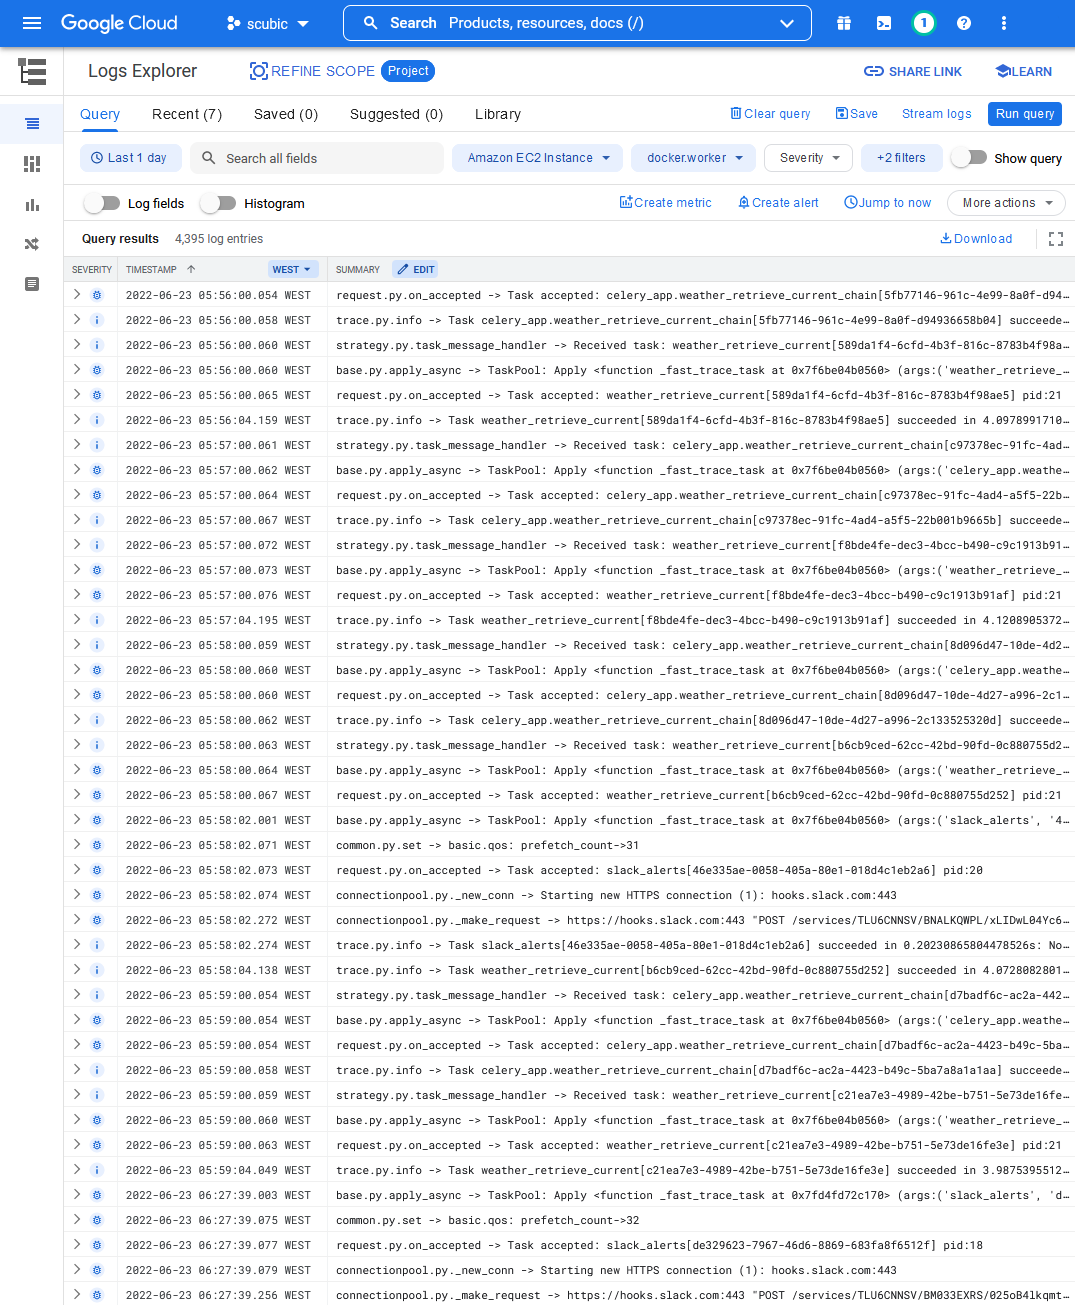
\includegraphics[width=0.97\textwidth]{img/screenshots/stackdriver-example-01.png}}
    \caption[Screenshot Google Cloud Log Monitoring]{Screenshot of an old Application's Worker's Logs displayed on the formerly named Stackdriver, now part of Google's Cloud solutions.}
    \label{fig:stackdriver-example-01}
\end{figure} 
    

\input{tex/contents/a2.tex}
\end{appendices}

% To make sure the document ends with an even number page.
\cleardoublepage

\end{document}
